Although the synchronization protocol is one of the defining factors in simulation performance, model allocation has a significant impact on which protocol is ideal.
Depending on the model structure, and how it is mapped to the different kernels, it might not even make sense to parallelize at all.
Indeed, if the model is distributed such that frequent communication is necessary between kernels, parallelism is naturally reduced.
This brings us to the topic of model allocation, as also implemented in \textit{PythonPDEVS}~\cite{PythonPDEVS2}.

The modeller can specify which kernel a model should be allocated to, should such manual intervention be required.
This is handled by the default model allocator.
If no preference is given, a simple striping scheme is used but this is often insufficient.
By overriding the default allocator, a modeller tunes the allocation scheme for a specific model, maximizing parallel speedup.
This interface can be linked to graph algorithms for automatic allocation scheme generation, for example to avoid cycles in the dependency graph.

\subsection{Performance Evaluation}
To evaluate the influence of model allocation, we define a new model, based on PHOLD~\cite{PHOLD}.
The model structure resembles a tree: an atomic model can have a set of children, with children being connected to each other recursively.

Unlike the Queue model, the width of the hierarchy is still present in the topology of the atomic models after direct connection.
The PHOLDTree model allows us to investigate parallel speedup in terms of model allocation, by modifying the depth and width (fanout) model parameters.

The PHOLDTree model is similar in structure to models of gossiping in social networks~\cite{Gossip}.
The lookahead of an atomic node is the minimally allowed $\epsilon$, indicating uncertainty, as is often the case in realistic models.
We demonstrate the importance of allocation by comparing performance of a breadth-first versus a depth-first scheme.
Both options are automated ways of allocation that are independent of the model.

\begin{figure}
    \center
    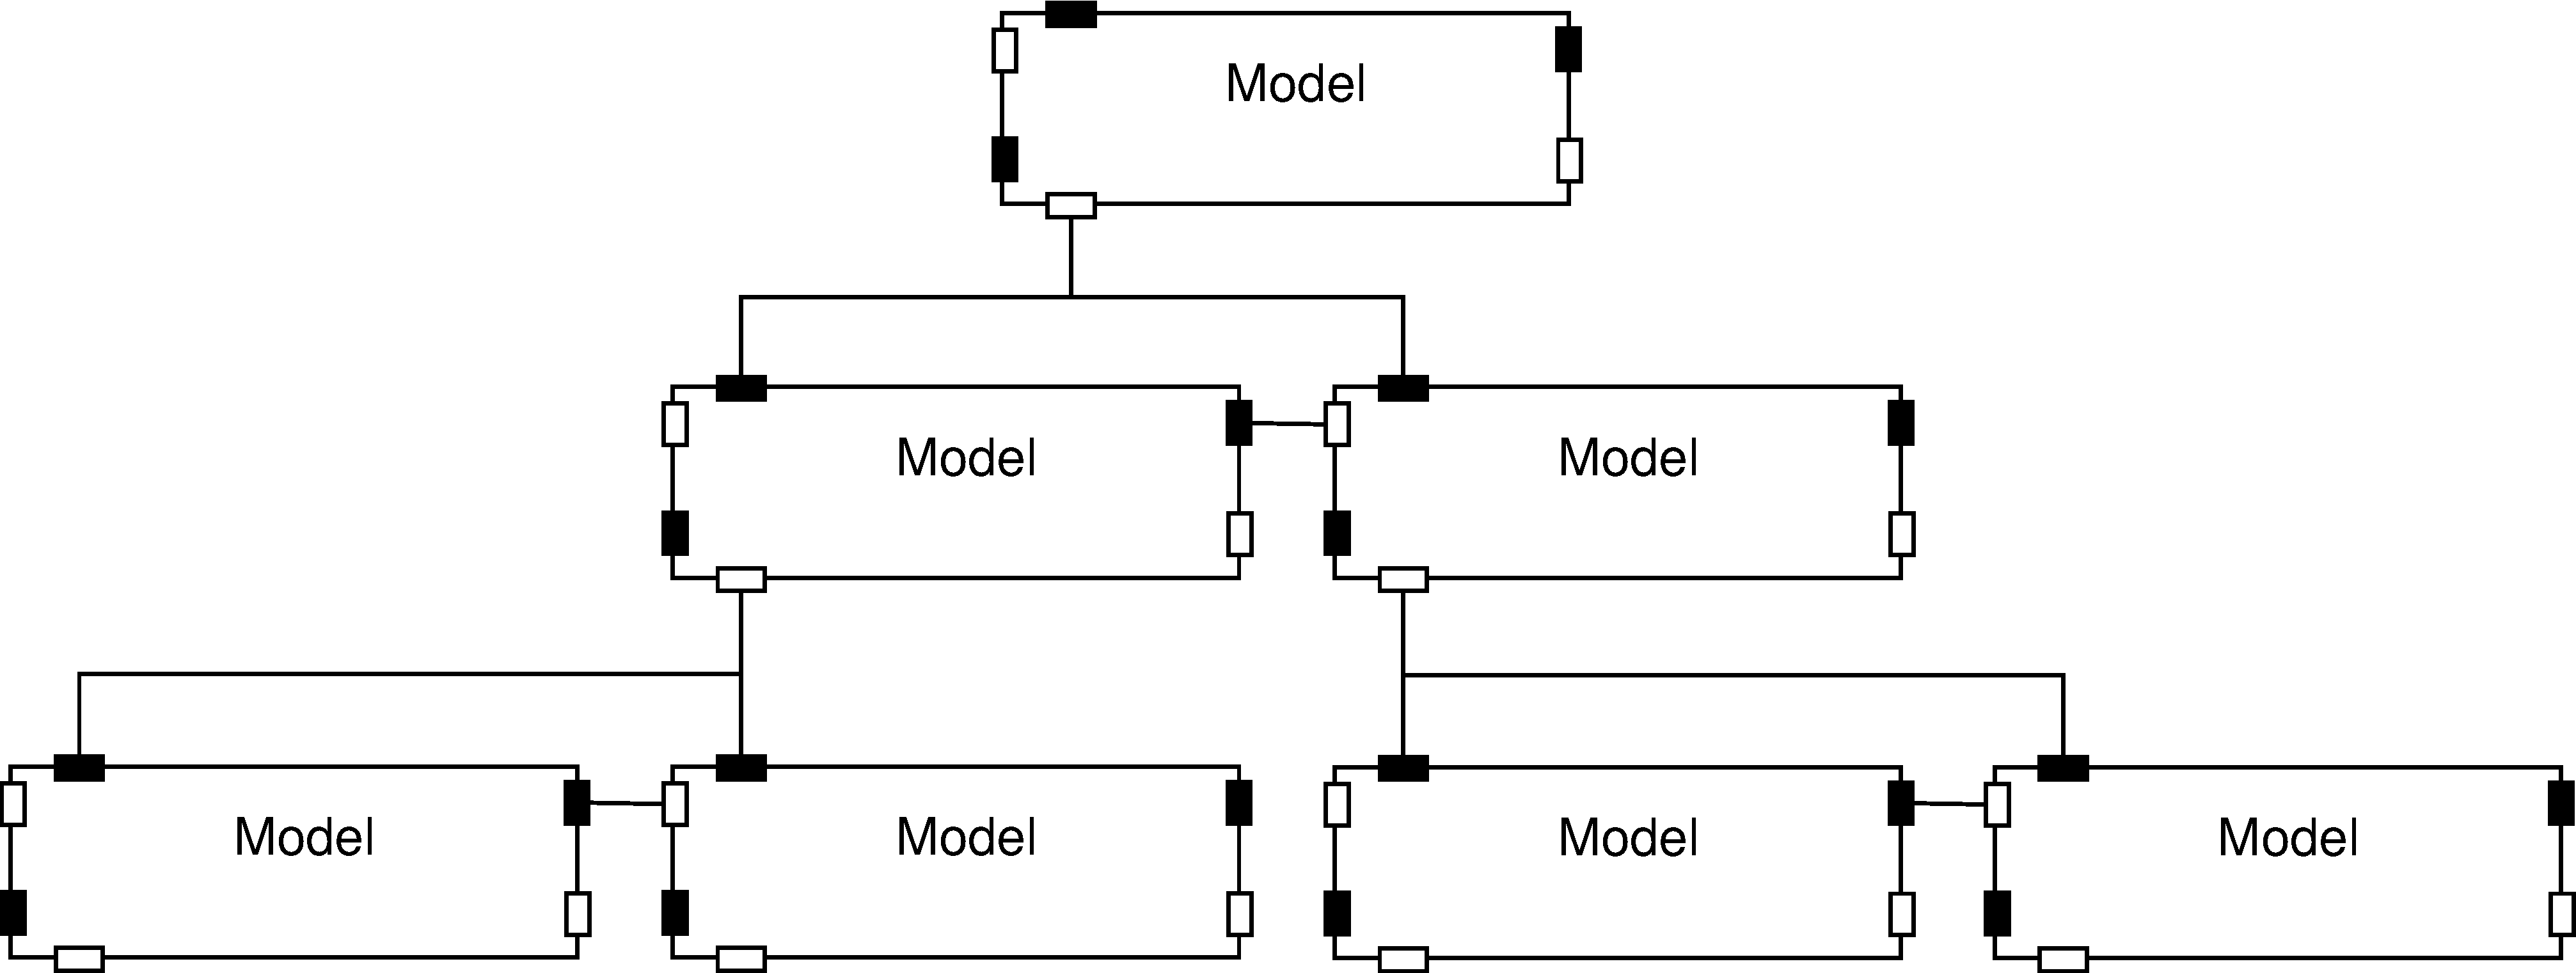
\includegraphics[width=\columnwidth]{fig/pholdtree.pdf}
    %TODO depth 1 but 3 levels deep?
    \caption{PHOLDTree model for depth 1 and width 2.}
    \label{fig:PHOLDTree_model}
\end{figure}

PHoldtree, like Queue, is a highly hierarchical model but one where the flattened structure cannot be partitioned into a chain, as was the case in the Queue model.
This topology is interesting since it highlights the effects of allocation.
First, we evaluate the model in sequential simulation to provide a baseline for parallel simulation.

\subsubsection{Sequential Simulation}
Since \textit{adevs} does not use direct connection, we expect a noticable performance difference between \textit{dxex} and \textit{adevs}.
This is shown in Figure~\ref{fig:PHOLDtree_seq_dn_benchmark}, where the fanout ($n$) determines the performance penalty \textit{adevs} suffers compared to \textit{dxex}.
Profiling indeed indicates that an increase in width per subtree ($n$) leads to higher overheads in \textit{adevs} due to the lack of direct connection.
\textit{Dxex} uses direct connection, making it independent on fanout.
Performance of \textit{dxex} is, in this model, only dependent on the number of models.
Slight deviations can still be seen, though, caused by the initialization overhead of direct connection.
Both \textit{adevs} and \textit{dxex} scale linearly in the number of atomic models.

\begin{figure}
    \center
    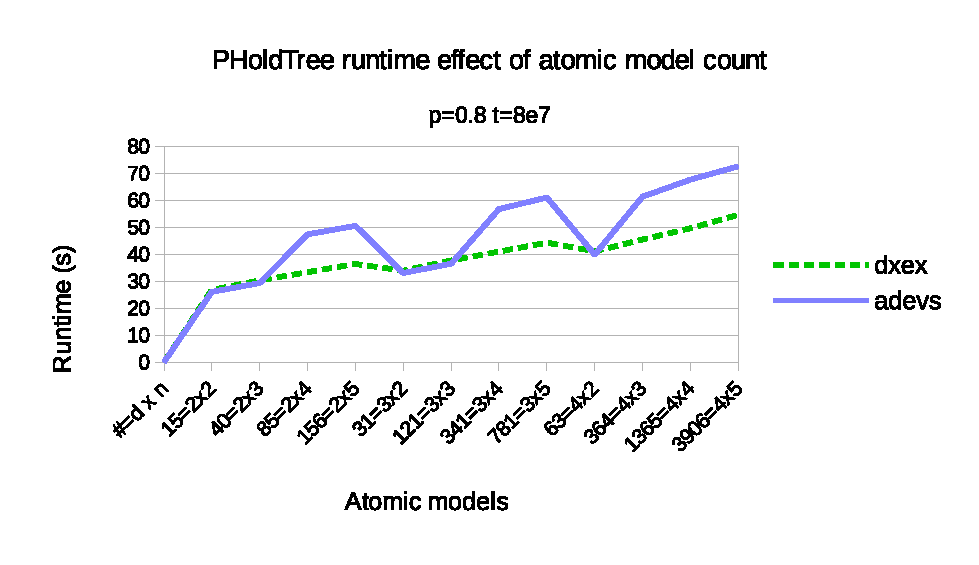
\includegraphics[width=\columnwidth]{fig/pholdtree_sequential_dn.eps}
    \caption{Effect of hierarchy in sequential simulation.}
    \label{fig:PHOLDtree_seq_dn_benchmark}
\end{figure}

\subsubsection{Parallel Simulation}
Next, we run the model using two different model allocation schemes: breadth-first and depth-first.
But first, we explain what we mean by both allocation schemes.

With breadth-first allocation, we traverse the tree in a breadth-first way, allocating subsequently visited atomic models to the same node.
This means, intuitively, that atomic models at the same level in the tree, but not necessarily siblings, are frequently allocated to the same node.
Since there is only infrequently some communication between siblings, and even never between different subtrees, this does not sound an intuitive allocation.
This allocation strategy is shown in Figure~\ref{fig:PholdTree_model_bfs}.

With depth-first allocation, we traverse the tree in a depth-first way, allocating subsequently visited atomic models to the same node.
This means, intuitively, that subtreees are frequently allocated to the same node.
This allocation strategy is shown in Figure~\ref{fig:PholdTree_model_dfs}.

Both allocators will try to divide models evenly over kernels. The effects of varying the number of models per kernel are already evaluated in the previous section on scaling. Here we want to highlight the overhead of communication and inter-kernel dependence. 

\begin{figure}
   \center
   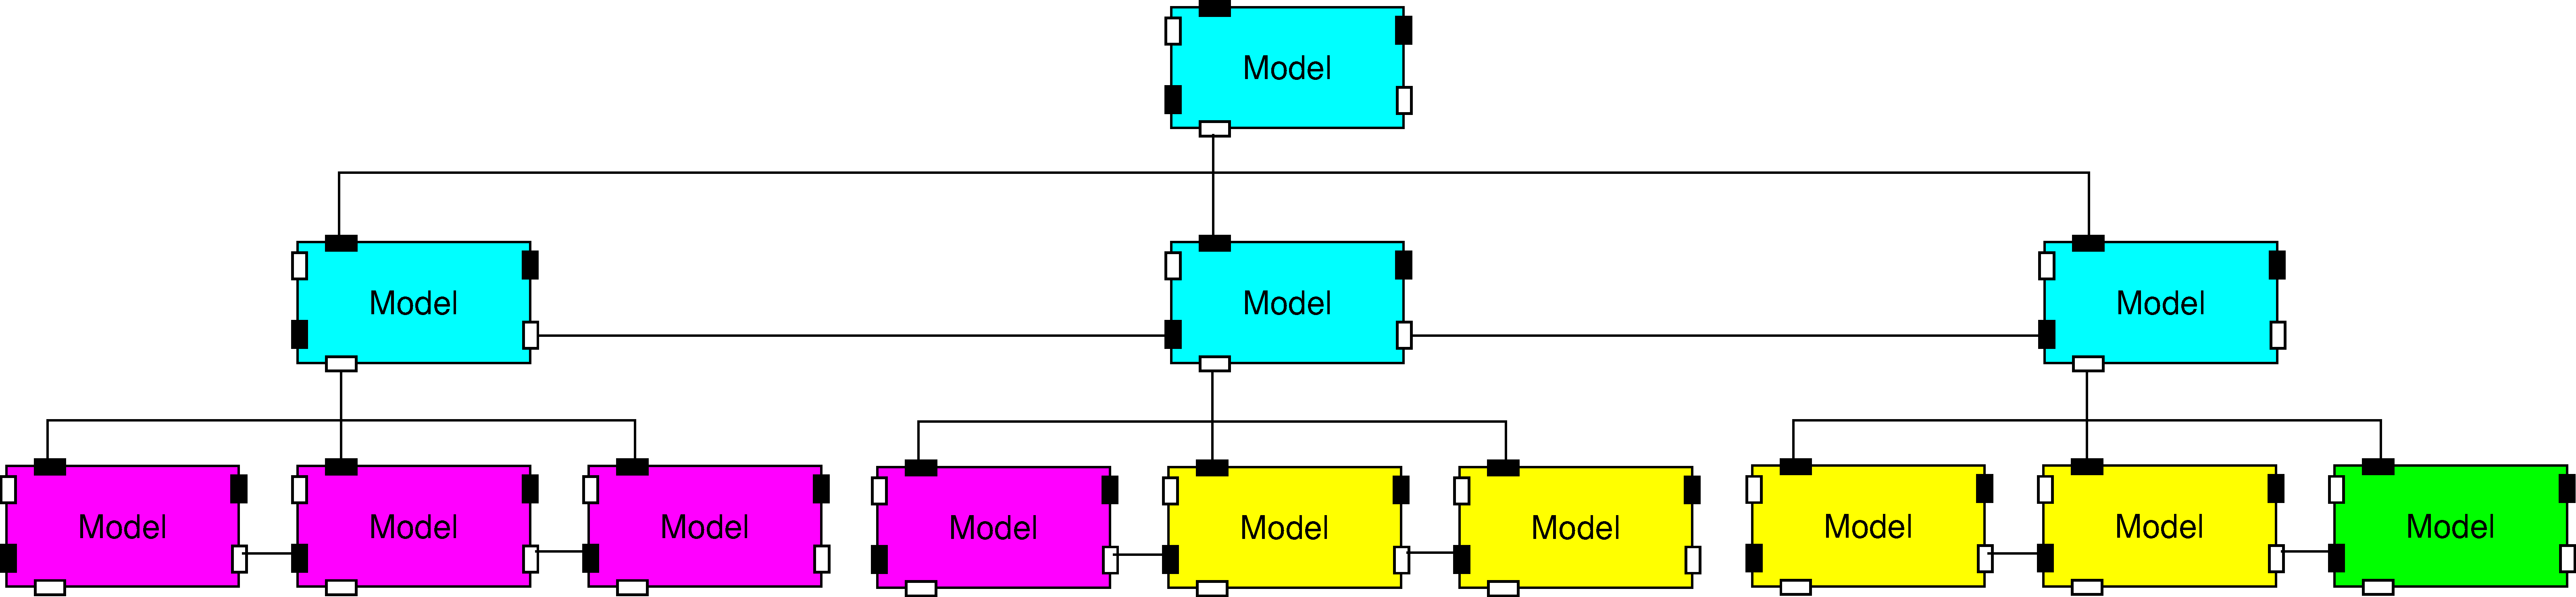
\includegraphics[width=\columnwidth]{fig/pholdtree_alloc_BF.pdf}
   \caption{PHOLDTree model breadth first allocation with 4 kernels.}
   \label{fig:PholdTree_model_bfs}
\end{figure}
\begin{figure}
   \center
   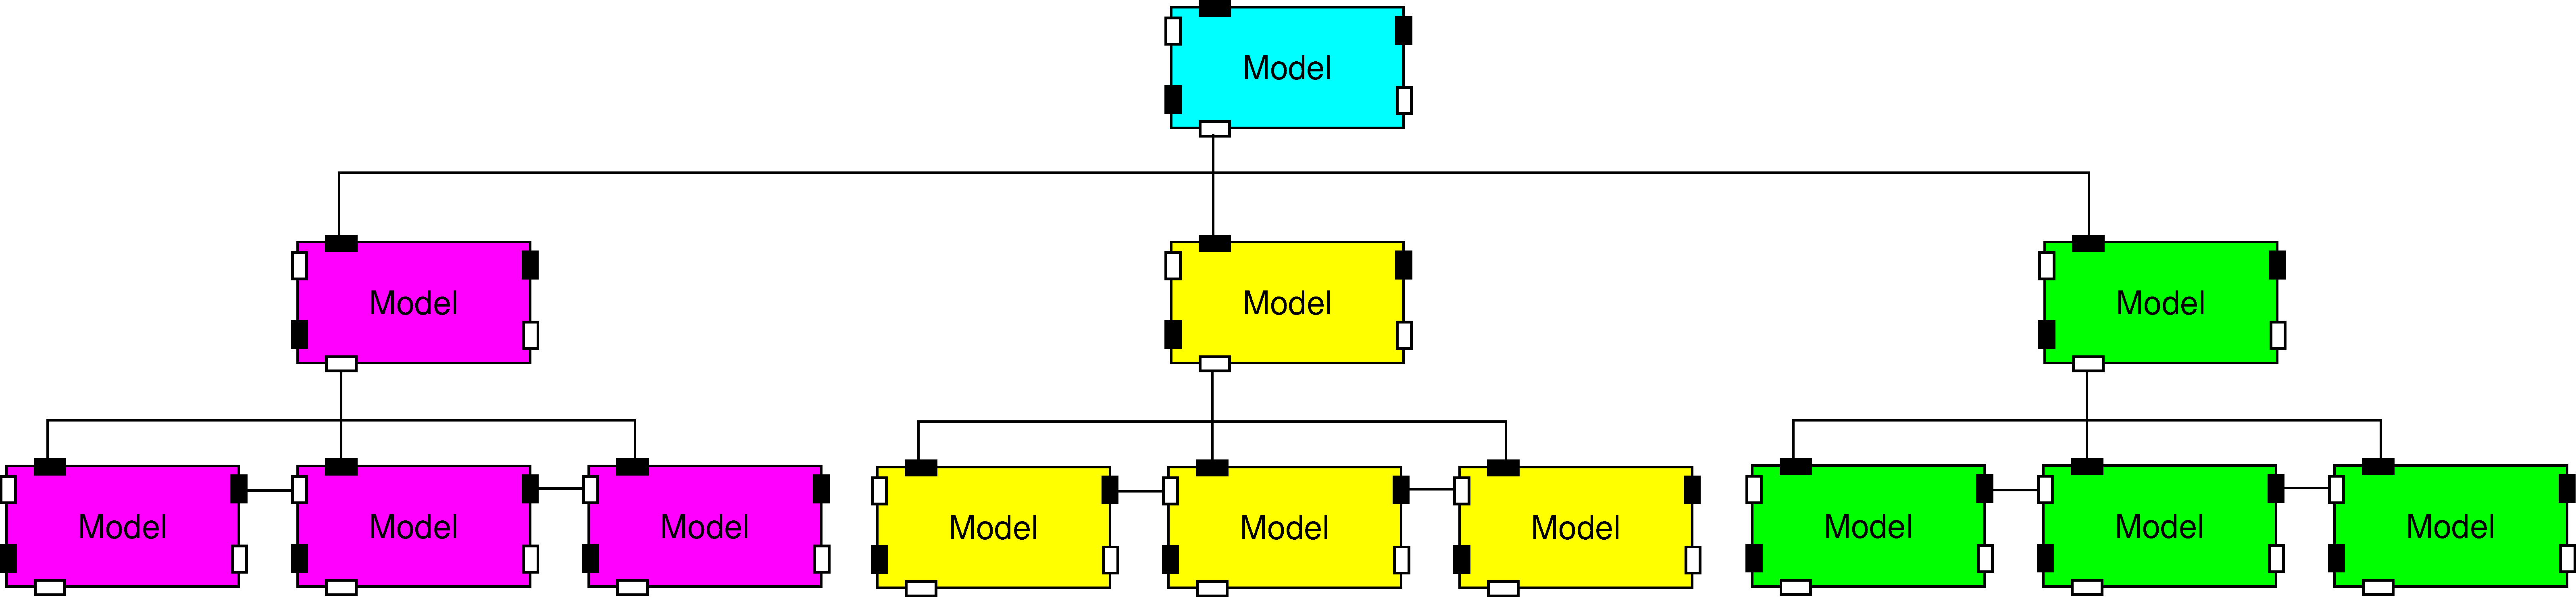
\includegraphics[width=\columnwidth]{fig/pholdtree_alloc_DF.pdf}
   \caption{PHOLDTree model depth first allocation with 4 kernels.}
   \label{fig:PholdTree_model_dfs}
\end{figure}

The breadth first allocation scheme results in a dependency chain with multiple branches, much like in the Queue model.
Such a linear dependency chain can result in a parallel speedup as we demonstrated with the Queue model.
This is not always true though: a single kernel with an unbalanced number of atomic models or unequal computational load in transition functions slows down the remainder of the chain.
This effect is also apparent if the thread a kernel runs on is not fairly scheduled.
With conservative synchronization this leads to excessive polling of the EOT of the other kernels.
With optimistic synchronization this leads to a cascade of rollbacks, since dependent kernels will simulate ahead of the slower kernel.

After simulation the traces can be visualized for both breadth-first and depth-first allocation.
Using a breadth-first allocation scheme, as shown in Figure~\ref{fig:pholdtree_visualize_parBFS}, we notice that many events get exchanged between kernels.
This is caused by the high number of inter-kernel connections and the high number of events exchanged over these connections.
The number of connections between nodes at the same simulation kernel is also rather low.
Using a depth-first allocation scheme, however, as shown in Figure~\ref{fig:pholdtree_visualize_parDFS}, minimizes inter-kernel connections while maximizing intra-kernel connections.

\begin{figure}
    \center
    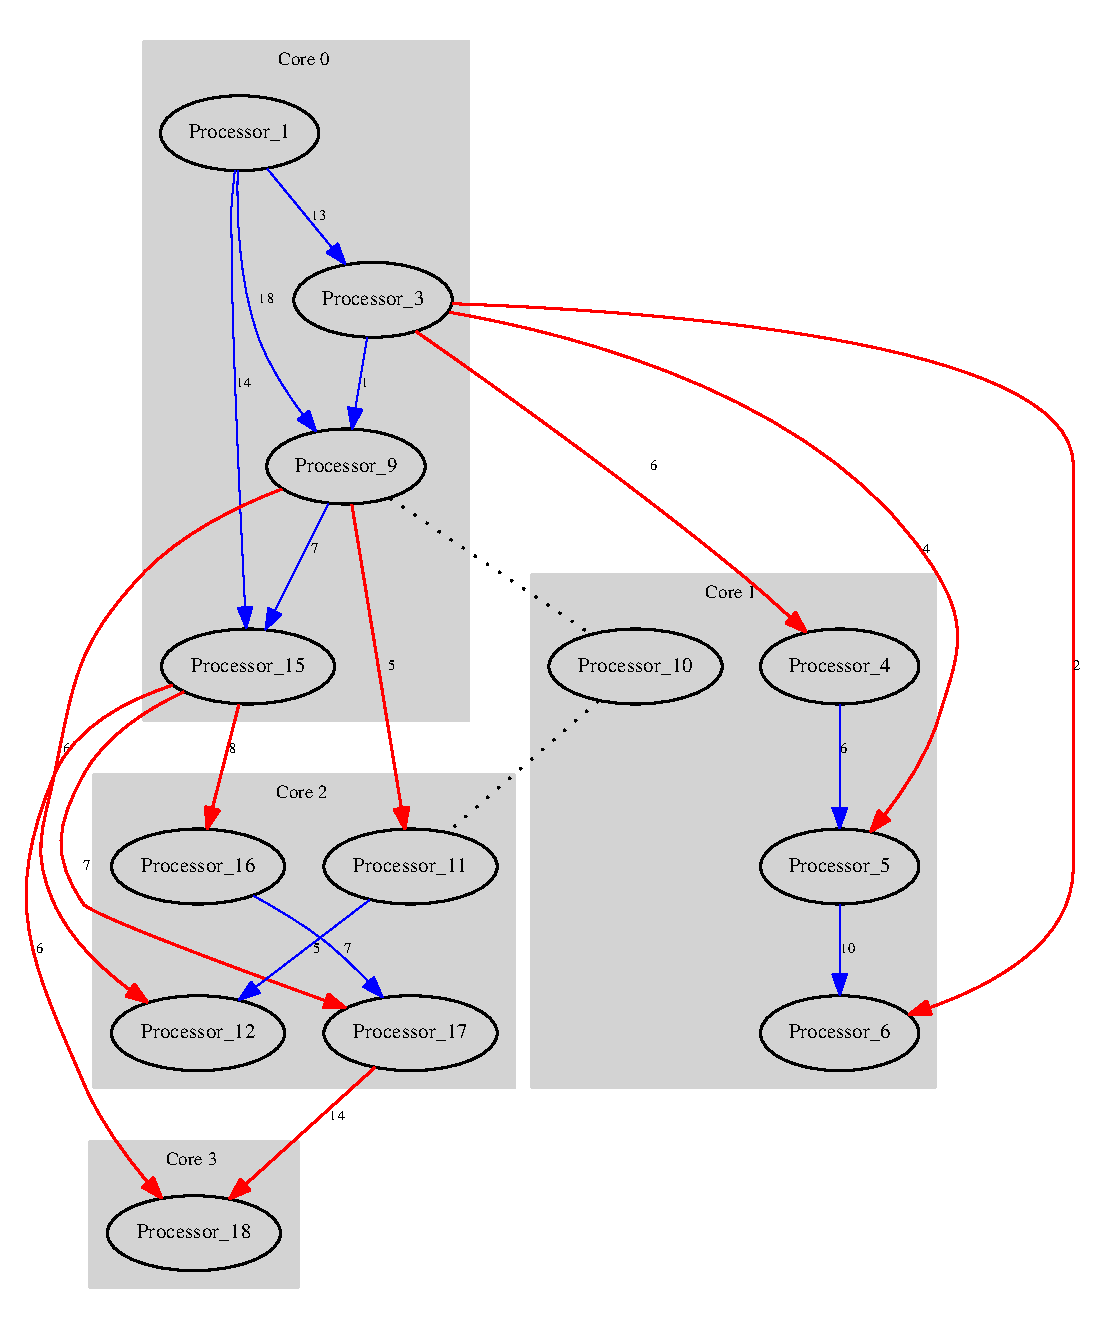
\includegraphics[width=\columnwidth]{fig/pholdtreed1n3t5000c4BFS.eps}
    \caption{Visualization of a PHOLDTree simulation with breadth first allocation and 4 kernels.}
    \label{fig:pholdtree_visualize_parBFS}
\end{figure}
\begin{figure}
    \center
    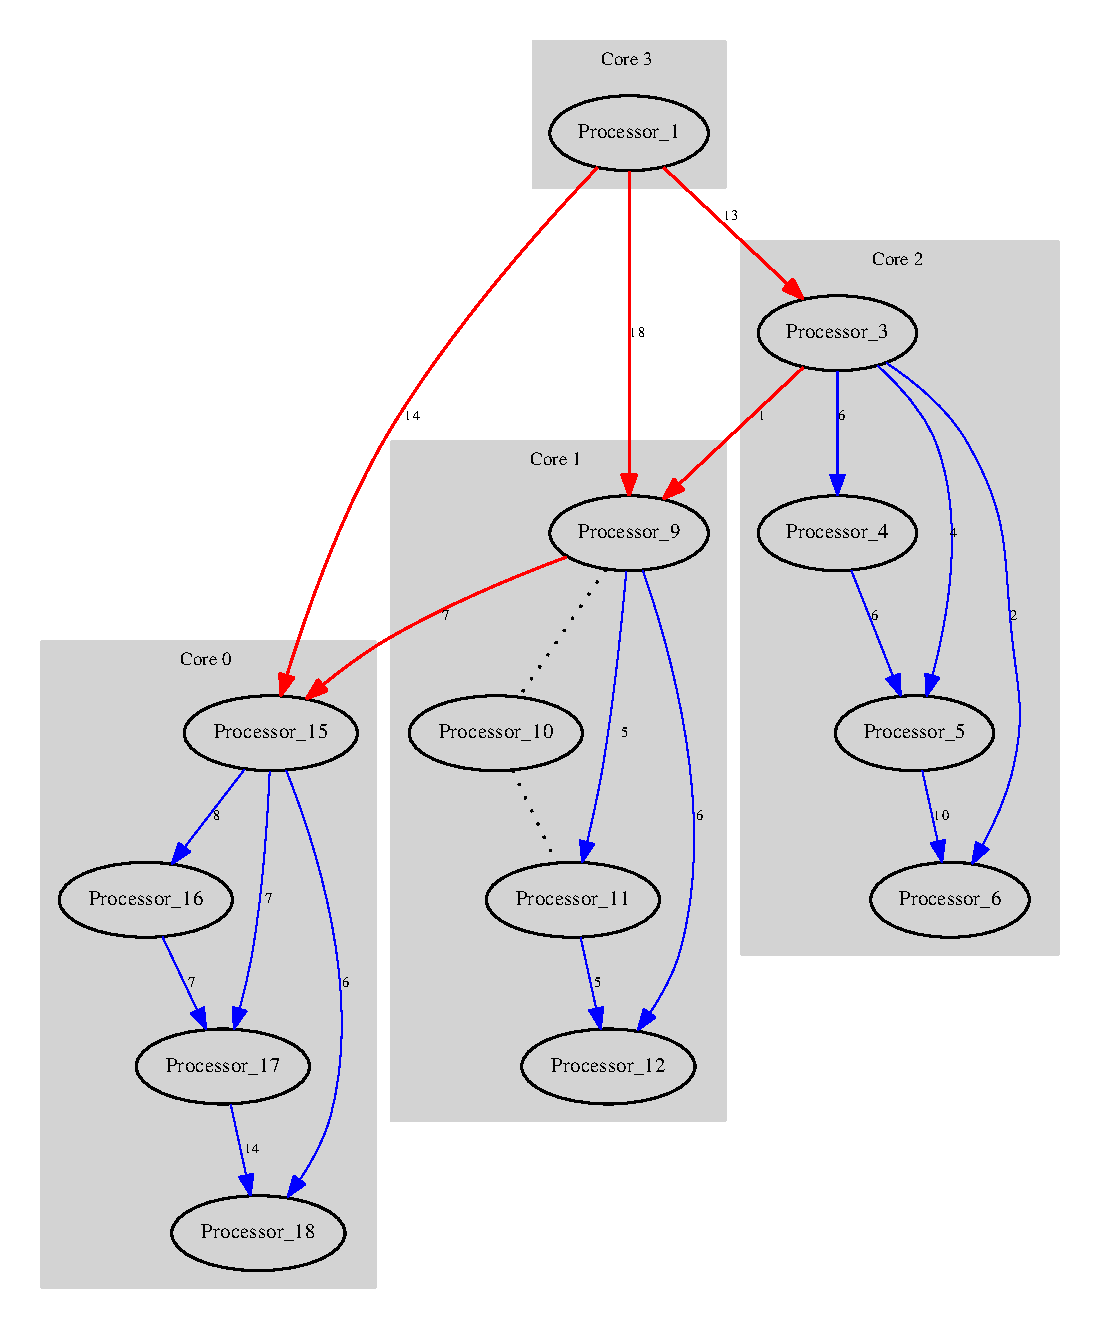
\includegraphics[width=\columnwidth]{fig/pholdtreed1n3t5000c4DFS.eps}
    \caption{Visualization of a PHOLDTree simulation with depth first allocation and 4 kernels.}
    \label{fig:pholdtree_visualize_parDFS}
\end{figure}

Simulation results are shown in Figure~\ref{fig:PholdTree_plot_alloc_high} for both allocation schemes in combination with both synchronization protocols.
We see that for both synchronization protocols, the depth-first allocation is significantly better than breadth-first allocation.
This is what we expected for this model: depth-first allocation maintains locality better than breadth-first allocation.
Whereas this is the case in this example, this is not true in general, as the ideal allocation depends on the model being simulated.

The most prominent aspect of these results is the low performance for conservative depth-first allocation for two kernels.
This is mostly caused by the difference between a sequential simulation and a parallel simulation: suddenly we need to take into account synchronization and passing around of lookahead values.
And since the number of kernels is low, the overhead dominates any further speedup.
Optimistic is less sensitive to the number of models per kernel as it does not need to poll each model for a lookahead, this explains the lower runtime penalty observed for optimistic.

%The effect is due to the topology of the kernels, in BFS the risk on reverts is higher. Optimistic is less influenced but will get a lower speedup in the good case.
Interestingly, we see that optimistic synchronization is less influenced by the allocation than conservative synchronization.
This is likely caused due to the lower number of connections to take into account in conservative synchronization.
Whereas conservative synchronization needs to take into account even scarcely used connections, optimistic synchronization does not.
The same is true in the opposite direction, though, where optimistic synchronization is slower when a good allocation is chosen.
Conservative synchronization will then be able to make better estimates, whereas optimistic synchronization does not make estimations. 

\begin{figure}
    \center
    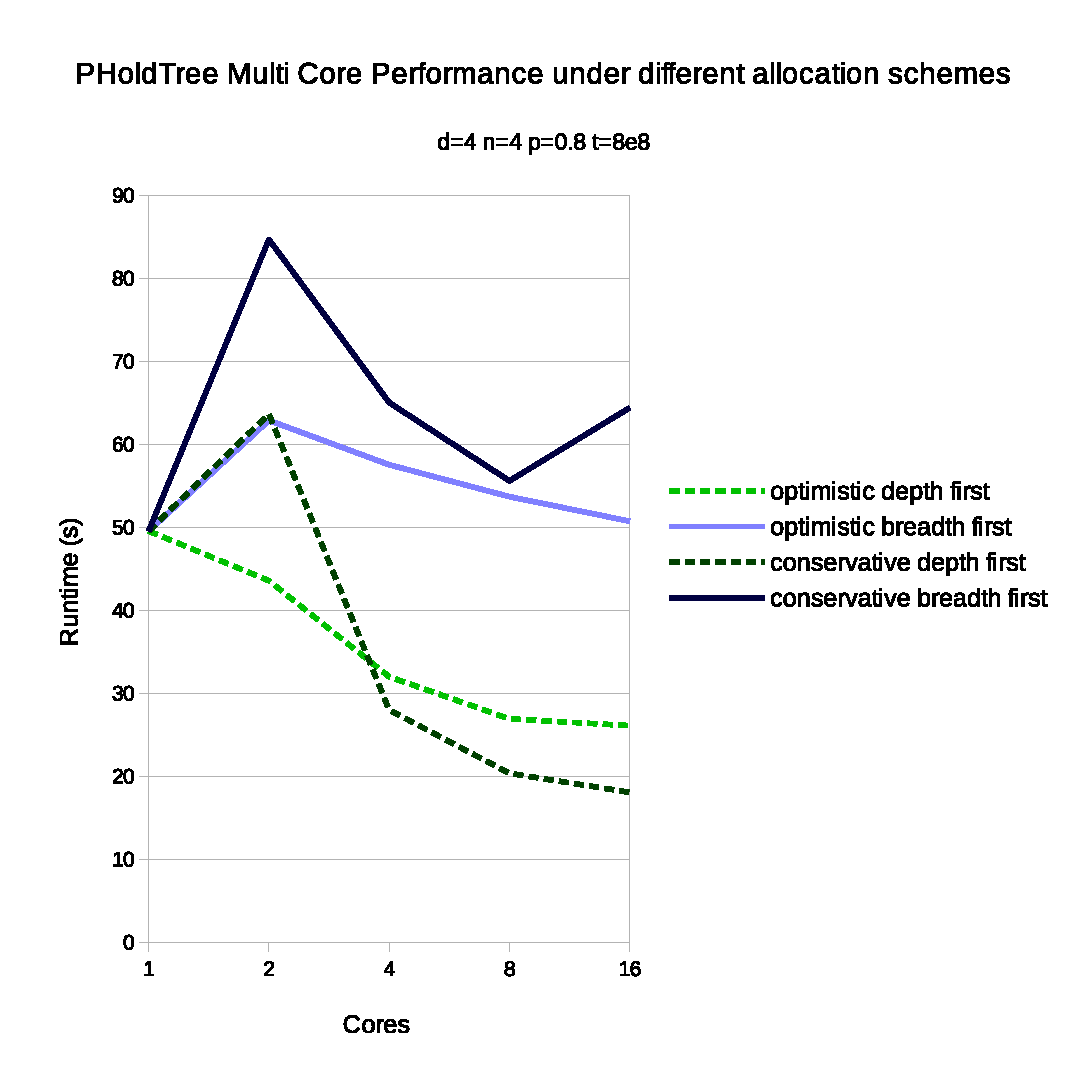
\includegraphics[width=\columnwidth]{fig/pholdtreeallochighp.eps}
    \caption{PHOLDTree model performance using different allocation schemes.}
    \label{fig:PholdTree_plot_alloc_high}
\end{figure}
